\documentclass{article}

% When submitting, replace this block with the venue style (e.g., neurips_2026.sty)
\usepackage[margin=1in]{geometry}
\usepackage[utf8]{inputenc}
\usepackage[T1]{fontenc}
\usepackage{hyperref}
\usepackage{url}
\usepackage{natbib}
\usepackage{booktabs}
\usepackage{amsfonts}
\usepackage{amsmath}
\usepackage{nicefrac}
\usepackage{microtype}
\usepackage{graphicx}
\usepackage{xcolor}
\usepackage{multirow}
\usepackage{subcaption}
\usepackage{tikz}
\usetikzlibrary{arrows.meta,positioning,calc,fit,backgrounds,decorations.pathreplacing}

\title{LOLM: Language Modeling Beyond the Surface\\with Hybrid Transformer-SSM Latent Order Fields}

\author{
  Bryan Leonard\thanks{Equal contribution.} \quad Brandyn Leonard\footnotemark[1] \\
  Qira LLC \\
  \texttt{bryanleonard237@gmail.com} \\
  \url{https://github.com/TheArtOfSound}
}

\begin{document}

\maketitle

%==============================================================================
\begin{abstract}
%==============================================================================
We introduce the \textbf{Latent Order Language Model (LOLM)}, a hybrid
architecture that augments a Transformer decoder with four parallel subsystems:
a selective state-space model (SSM) for tracking slow latent dynamics, a
persistent three-bank external memory, a discrete regime layer with
Gumbel-Softmax phase detection, and a learned per-dimension manifestation gate
that arbitrates between surface and latent representations. The central thesis
is that natural language is the \emph{surface manifestation} of deeper latent
cognitive processes---planning, discourse tracking, topic management---and that
explicitly modeling this separation yields more parameter-efficient language
models. At 304M parameters, LOLM achieves a perplexity of 68.37 on
WikiText-103, outperforming Pythia-410M (142.93 PPL) by 52.2\% at matched
compute despite having 26\% fewer parameters. At 1.57B parameters, LOLM
achieves 33.2 PPL on FineWeb-Edu versus 39.1 for a matched-budget
decoder-only baseline---a 15\% improvement confirming the architecture's
advantage under controlled comparison. Inference-time ablations confirm that
all novel components contribute meaningfully: at 1.57B, removing the latent
SSM path causes perplexity to explode from 34.5 to 485 million---a
$14{,}000{,}000\times$ increase despite the latent path comprising only
${\sim}30\%$ of the fused representation. Cross-hardware validation on
Google Cloud TPU v4 confirms the convergence advantage transfers: LOLM
converges up to 43\% faster than a parameter-matched baseline (317M
decoder-only, 200-step averaged PPL) during the first 15{,}000 steps,
with the baseline gradually closing the gap and reaching comparable
performance by 50{,}000 steps---consistent with a sample-efficiency
interpretation of the hybrid architecture.
We release all code and weights under the LOLM Community License.
\end{abstract}

%==============================================================================
\section{Introduction}
\label{sec:intro}
%==============================================================================

Modern language models operate on a single representational stream: tokens are
embedded, contextualized through self-attention or recurrence, and projected
back to vocabulary space. This architecture implicitly assumes that all
information relevant to next-token prediction can be captured in a single hidden
state at each position. Yet cognitive science and discourse analysis suggest
that human language production involves multiple concurrent processes at
different timescales: fast surface-level word selection, medium-speed syntactic
planning, and slow discourse-level topic and intent management
\citep{pickering2004toward,kintsch1998comprehension}.

We propose the \textbf{Latent Order Language Model (LOLM)}, which explicitly
separates language modeling into a \emph{surface stream} (standard Transformer
decoder) and a \emph{latent order field} (selective SSM + persistent memory +
discrete regime detection). A learned \emph{manifestation gate} dynamically
determines, at each token position and each hidden dimension, how much of the
output should be driven by surface-level vs.\ latent-order representations.

LOLM is motivated by the observation that certain aspects of language---topic
coherence, narrative planning, argumentation structure---evolve on timescales
much longer than the attention window of any practical Transformer. While SSMs
like Mamba \citep{gu2023mamba} excel at long-range dependencies through
recurrent state, they lack the discrete mode-switching that characterizes human
discourse (e.g., shifting from exposition to argumentation). LOLM bridges this
gap with a \emph{regime layer} that performs discrete phase detection via
Gumbel-Softmax \citep{jang2016categorical}, producing spatially coherent regime
segments through causal convolution over regime logits.

Our contributions are:
\begin{enumerate}
    \item A novel hybrid architecture combining Transformers, selective SSMs,
    persistent memory, discrete regime detection, and learned gating in a
    unified language model.
    \item A multi-objective training framework with seven complementary losses,
    including contrastive predictive coding (CPC) for the latent SSM,
    changepoint-aligned regime diversity, and competitive gate training.
    \item Gradient isolation for discrete code selection, solving the persistent
    regime collapse problem that plagues discrete-bottleneck architectures.
    \item Empirical results showing LOLM-304M outperforms Pythia-410M at
    matched compute and LOLM-1.57B outperforms a matched-budget baseline by
    15\%, with ablations confirming all components contribute meaningfully.
\end{enumerate}

%==============================================================================
\section{Related Work}
\label{sec:related}
%==============================================================================

\paragraph{State-Space Models for Language.}
Structured SSMs \citep{gu2021efficiently} and their selective variants
\citep{gu2023mamba} have demonstrated competitive language modeling with linear
time complexity. Mamba-2 \citep{dao2024transformers} further bridges SSMs and
attention. LOLM differs by using the SSM as a \emph{parallel} latent-order
tracker rather than a replacement for attention, gated by a learned arbitration
mechanism.

\paragraph{Hybrid Architectures.}
Jamba \citep{lieber2024jamba} interleaves Transformer and Mamba layers
sequentially. Griffin \citep{de2024griffin} combines gated linear recurrences
with local attention. LOLM takes a fundamentally different approach: the
Transformer and SSM operate on the same input in parallel, producing competing
representations that are arbitrated by a learned gate.

\paragraph{Memory-Augmented Language Models.}
Neural Turing Machines \citep{graves2014neural}, Memorizing Transformers
\citep{wu2022memorizing}, and $k$NN-LM \citep{khandelwal2020generalization}
augment language models with external memory. LOLM's persistent memory is
distinctive in using three semantically separated banks (episodic, semantic,
self-model) with gated read/write and chunked intra-sequence updates to
maintain gradient flow.

\paragraph{Discrete Codes in Neural Networks.}
VQ-VAE \citep{van2017neural} and mixture-of-experts \citep{shazeer2017moe}
use discrete bottlenecks. LOLM's regime layer shares the challenge of code
collapse; we solve it with gradient isolation (detaching regime embeddings from
the token loss), analogous to VQ-VAE's stop-gradient, combined with
MPST-inspired \citep{leonard2024mpst} neighbor interactions.

%==============================================================================
\section{Architecture}
\label{sec:architecture}
%==============================================================================

Figure~\ref{fig:architecture} illustrates the LOLM dataflow. Given a token
sequence $\mathbf{x} = (x_1, \ldots, x_T)$, the model produces logits via:

\begin{equation}
\label{eq:fusion}
\mathbf{o}_t = g_t \odot \text{LN}(W_h \mathbf{h}_t) + (1 - g_t) \odot \text{LN}(W_z \mathbf{z}_t) + W_m \mathbf{m}_t + W_r \bar{\mathbf{r}}_t
\end{equation}

where $\mathbf{h}_t$ is the surface decoder output, $\mathbf{z}_t$ the latent
SSM state, $\mathbf{m}_t$ the memory readout, $\bar{\mathbf{r}}_t$ the
(detached) regime embedding, $g_t \in [0,1]^d$ the manifestation gate, and
$\text{LN}$ denotes layer normalization. Logits are computed as $\ell_t = W_E^\top \mathbf{o}_t$ via weight tying with the token embedding $W_E$.

\begin{figure}[t]
\centering
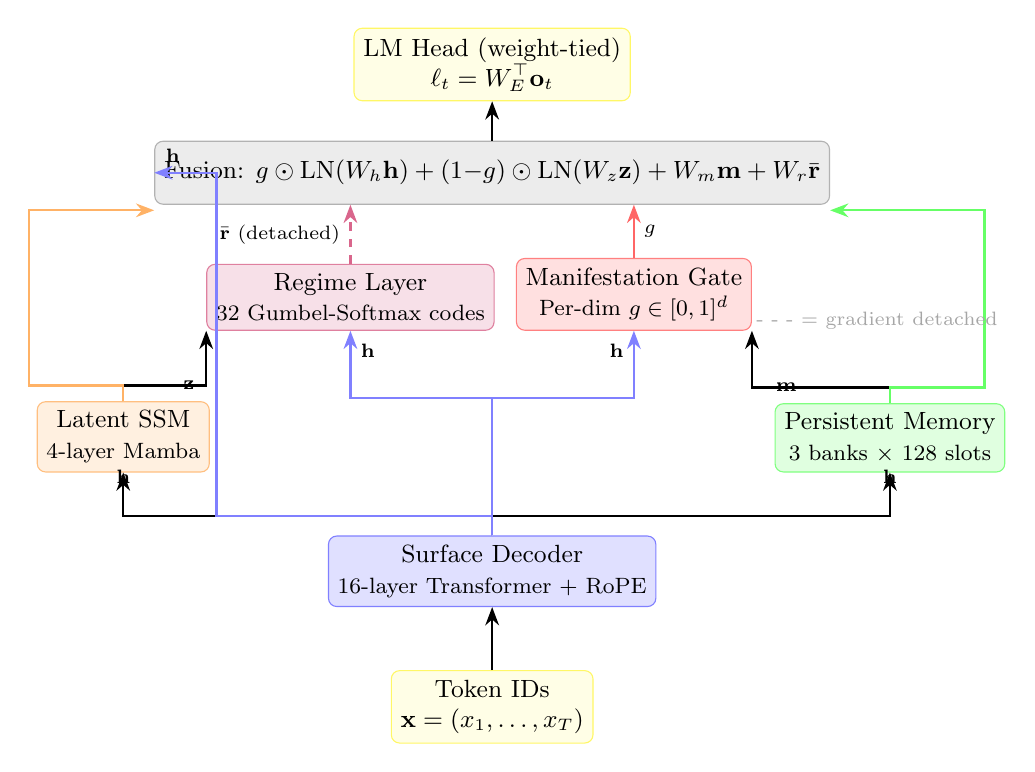
\begin{tikzpicture}[
    >=Stealth,
    node distance=0.6cm and 1.2cm,
    block/.style={draw, rounded corners=3pt, minimum height=0.8cm, minimum width=2.0cm, align=center, font=\small},
    surface/.style={block, fill=blue!12, draw=blue!50},
    latent/.style={block, fill=orange!12, draw=orange!50},
    memory/.style={block, fill=green!12, draw=green!50},
    regime/.style={block, fill=purple!12, draw=purple!50},
    gate/.style={block, fill=red!12, draw=red!50},
    fusion/.style={block, fill=gray!15, draw=gray!60, minimum width=5.4cm},
    io/.style={block, fill=yellow!10, draw=yellow!60},
    arr/.style={->, thick, >=Stealth},
    darr/.style={->, thick, >=Stealth, dashed, draw=gray!70},
]

% Input
\node[io] (input) {Token IDs\\$\mathbf{x} = (x_1, \ldots, x_T)$};

% Surface Decoder
\node[surface, above=0.8cm of input] (decoder) {Surface Decoder\\{\footnotesize 16-layer Transformer + RoPE}};

% Four parallel subsystems
\node[latent, above left=0.8cm and 1.5cm of decoder] (ssm) {Latent SSM\\{\footnotesize 4-layer Mamba}};
\node[memory, above right=0.8cm and 1.5cm of decoder] (mem) {Persistent Memory\\{\footnotesize 3 banks $\times$ 128 slots}};

% Regime and Gate (middle level)
\node[regime, above=2.6cm of decoder, xshift=-1.8cm] (regime) {Regime Layer\\{\footnotesize 32 Gumbel-Softmax codes}};
\node[gate, above=2.6cm of decoder, xshift=1.8cm] (gate_node) {Manifestation Gate\\{\footnotesize Per-dim $g \in [0,1]^d$}};

% Fusion
\node[fusion, above=4.2cm of decoder] (fuse) {Fusion: $g \odot \mathrm{LN}(W_h \mathbf{h}) + (1{-}g) \odot \mathrm{LN}(W_z \mathbf{z}) + W_m \mathbf{m} + W_r \bar{\mathbf{r}}$};

% Output
\node[io, above=0.5cm of fuse] (output) {LM Head (weight-tied)\\$\ell_t = W_E^\top \mathbf{o}_t$};

% Arrows: input -> decoder
\draw[arr] (input) -- (decoder);

% Arrows: decoder -> subsystems
\draw[arr] (decoder.north) -- ++(0, 0.25) -| (ssm.south) node[pos=0.75, above, font=\scriptsize] {$\mathbf{h}$};
\draw[arr] (decoder.north) -- ++(0, 0.25) -| (mem.south) node[pos=0.75, above, font=\scriptsize] {$\mathbf{h}$};

% Arrows: subsystems -> regime and gate
\draw[arr] (ssm.north) -- ++(0, 0.2) -| (regime.south west) node[pos=0.3, right, font=\scriptsize] {$\mathbf{z}$};
\draw[arr] (mem.north) -- ++(0, 0.2) -| (gate_node.south east) node[pos=0.3, left, font=\scriptsize] {$\mathbf{m}$};
\draw[arr, draw=blue!50] (decoder.north) -- ++(0, 0.25) -- ++(0, 1.5) -| (regime.south) node[pos=0.85, right, font=\scriptsize] {$\mathbf{h}$};
\draw[arr, draw=blue!50] (decoder.north) -- ++(0, 0.25) -- ++(0, 1.5) -| (gate_node.south) node[pos=0.85, left, font=\scriptsize] {$\mathbf{h}$};

% Arrows: all -> fusion
\draw[arr, draw=blue!50] (decoder.north) -- ++(0, 0.25) -- ++(-3.5, 0) |- (fuse.west) node[pos=0.85, above, font=\scriptsize] {$\mathbf{h}$};
\draw[arr, draw=orange!60] (ssm.north) -- ++(0, 0.2) -- ++(-1.2, 0) |- ([yshift=-2pt]fuse.south west) node[pos=0.6, above, font=\scriptsize] {};
\draw[arr, draw=green!60] (mem.north) -- ++(0, 0.2) -- ++(1.2, 0) |- ([yshift=-2pt]fuse.south east) node[pos=0.6, above, font=\scriptsize] {};
\draw[darr, draw=purple!60] (regime.north) -- ([xshift=-1.8cm]fuse.south) node[midway, left, font=\scriptsize] {$\bar{\mathbf{r}}$ (detached)};
\draw[arr, draw=red!60] (gate_node.north) -- ([xshift=1.8cm]fuse.south) node[midway, right, font=\scriptsize] {$g$};

% Fusion -> output
\draw[arr] (fuse) -- (output);

% Legend for detached
\node[anchor=west, font=\scriptsize, text=gray!70] at ([xshift=3.2cm, yshift=-0.3cm]regime.east) {- - - = gradient detached};

\end{tikzpicture}
\caption{\textbf{LOLM architecture.} Token IDs pass through the Surface
Decoder to produce hidden states $\mathbf{h}$. Four parallel subsystems
process $\mathbf{h}$: the Latent SSM ($\mathbf{z}$), Persistent Memory
($\mathbf{m}$), Regime Layer ($\bar{\mathbf{r}}$, gradient-detached), and
Manifestation Gate ($g$). The fusion layer combines all representations via
per-dimension gating and additive contributions. The LM head shares weights
with the token embedding.}
\label{fig:architecture}
\end{figure}

%--------------------------------------
\subsection{Surface Decoder}
\label{sec:decoder}
%--------------------------------------

The surface decoder is a pre-norm Transformer \citep{xiong2020layer} with
Rotary Position Embeddings (RoPE) \citep{su2024roformer}. Each of $L$ layers
applies multi-head self-attention with causal masking followed by a
position-wise feed-forward network with GELU activation:

\begin{align}
\mathbf{h}^{(l)} &= \mathbf{h}^{(l-1)} + \text{MHA}(\text{LN}(\mathbf{h}^{(l-1)})) \\
\mathbf{h}^{(l)} &= \mathbf{h}^{(l)} + \text{FFN}(\text{LN}(\mathbf{h}^{(l)}))
\end{align}

At the 304M scale: $d = 1024$, $L = 16$ layers, 16 attention heads, $d_\text{ff} = 4096$.

%--------------------------------------
\subsection{Latent SSM Core}
\label{sec:ssm}
%--------------------------------------

The latent SSM processes the decoder's hidden states $\mathbf{h}$ through $K$
layers of selective state-space recurrence (Mamba-style) \citep{gu2023mamba}.
Each layer computes input-dependent discretization:

\begin{align}
\Delta_t &= \text{softplus}(W_\Delta \mathbf{x}_t + b_\Delta) \\
\bar{A}_t &= \exp(\Delta_t \cdot A), \quad \bar{B}_t = \Delta_t \cdot (W_B \mathbf{x}_t) \\
\mathbf{s}_t &= \bar{A}_t \odot \mathbf{s}_{t-1} + \bar{B}_t \odot \mathbf{x}_t \\
\mathbf{z}_t &= (W_C \mathbf{x}_t) \cdot \mathbf{s}_t
\end{align}

where $A$ is a learned diagonal matrix (parameterized in log-space for
stability), and $\mathbf{s}_t \in \mathbb{R}^{d_\text{inner} \times d_\text{state}}$ is the recurrent state. Output gating via SiLU and skip connections follow Mamba.

We implement three scan backends: CUDA kernels from \texttt{mamba-ssm} (primary), a memory-efficient custom autograd scan using reverse-pass reconstruction (saving $\mathcal{O}(T \log T)$ memory vs.\ parallel scan autograd), and a parallel associative scan fallback. At the 304M scale: $K=4$ layers, $d_\text{state}=32$, expand factor 2 ($d_\text{inner}=2048$).

The SSM operates on the decoder's already-contextualized representations rather
than raw embeddings, allowing it to track \emph{latent dynamics}---slow semantic drift, unresolved plans, topic evolution---that the attention layers have partially resolved.

%--------------------------------------
\subsection{Persistent Memory}
\label{sec:memory}
%--------------------------------------

LOLM maintains three external memory banks---\emph{episodic}, \emph{semantic},
and \emph{self-model}---each containing $N$ learnable slot vectors
$M \in \mathbb{R}^{N \times d_s}$. At each position, the model reads via
scaled dot-product attention:

\begin{equation}
\text{read}_t = \text{softmax}\!\left(\frac{W_q \mathbf{h}_t \cdot M^\top}{\sqrt{d_s}}\right) M
\end{equation}

Reads from all three banks are concatenated and projected to $d$-dimensions.
Memory is updated via gated writes aggregated over sequence chunks:

\begin{equation}
M' = \alpha \odot M + \beta \odot W_c \bar{\mathbf{h}}, \quad
\alpha = \sigma(W_\alpha \bar{\mathbf{h}}), \quad
\beta = \sigma(W_\beta \bar{\mathbf{h}})
\end{equation}

where $\bar{\mathbf{h}}$ is the chunk-averaged hidden state. The forget gate
$\alpha$ and write gate $\beta$ operate per-slot, analogous to LSTM gating.

\paragraph{Chunked processing.} To create gradient flow through the write
mechanism, each sequence is split into $C$ chunks. Chunk $i$'s write updates
the memory that chunk $i{+}1$ reads from, establishing the path
$\mathcal{L} \to \text{read}_{i+1} \to M_i \to \text{write}_i \to W_\text{write}$.
Without chunking, write parameters receive zero gradient. At the 304M scale:
$N=128$ slots per bank, $d_s=1024$, $C=4$ chunks.

%--------------------------------------
\subsection{Regime Layer}
\label{sec:regime}
%--------------------------------------

The regime layer performs discrete phase detection, assigning each token
position a soft distribution over $R$ regime codes via Gumbel-Softmax:

\begin{equation}
\mathbf{p}_t = \text{GumbelSoftmax}\!\left(
    \text{clamp}\!\left(
        W_\ell [\mathbf{z}_t; \mathbf{h}_t; \mathbf{m}_t] + \gamma \cdot \text{Conv1d}_\text{causal}(\boldsymbol\ell),\;
        [-5, 5]
    \right),\; \tau
\right)
\end{equation}

where $\boldsymbol\ell$ denotes the raw logits before neighbor interaction,
$\gamma$ is a learned scaling parameter (initialized to 0.1), and the causal
Conv1d (kernel size 7) creates spatially coherent regime segments by allowing
adjacent tokens to influence each other's regime selection. This is inspired by
the Ising-model dynamics of Multi Phase Selection Tool (MPST), where
local interactions and stochastic noise drive emergent phase boundaries.

The regime embedding is $\mathbf{r}_t = \mathbf{p}_t \cdot E_r$ where
$E_r \in \mathbb{R}^{R \times d_r}$ is a learnable codebook. At the 304M
scale: $R=32$ codes, $d_r=128$, $\tau$ annealed from 1.0 to 0.5 over 150K
steps.

\paragraph{Gradient isolation.} The regime embedding $\mathbf{r}_t$ is
\emph{detached} before entering the fusion (Eq.~\ref{eq:fusion}). The regime
layer is trained exclusively by its own losses (Section~\ref{sec:regime_loss}).
This prevents the token prediction gradient from collapsing all codes into a
single mode that minimizes cross-entropy---a failure mode we consistently
observed without isolation (Section~\ref{sec:ablation_collapse}).

%--------------------------------------
\subsection{Manifestation Gate}
\label{sec:gate}
%--------------------------------------

The manifestation gate produces a per-dimension mixing coefficient
$g_t \in [0,1]^d$ via a two-layer MLP:

\begin{equation}
g_t = \sigma\!\left(W_2 \cdot \text{GELU}(W_1 [\mathbf{z}_t; \mathbf{h}_t; \mathbf{m}_t; \mathbf{r}_t]) + b_2\right)
\end{equation}

where $b_2$ is initialized to $-0.5$, biasing the gate toward $g \approx 0.38$
(latent-preferring) at initialization. The gate is \emph{per-dimension} rather
than scalar, allowing different feature dimensions to draw from different
sources. Both branches are layer-normalized before gating to prevent magnitude
mismatch (Eq.~\ref{eq:fusion}).

%==============================================================================
\section{Training}
\label{sec:training}
%==============================================================================

%--------------------------------------
\subsection{Multi-Objective Loss}
\label{sec:losses}
%--------------------------------------

LOLM is trained with seven loss terms:

\begin{equation}
\mathcal{L} = \mathcal{L}_\text{tok} + \sum_{i} \lambda_i \mathcal{L}_i
\end{equation}

\paragraph{Token cross-entropy ($\mathcal{L}_\text{tok}$).}
Standard next-token prediction, computed in chunks of 4096 positions to avoid
materializing the full $(BT \times V)$ logit tensor in float32 (which would
require ${\sim}12$\,GB at our batch size).

\paragraph{Contrastive predictive coding ($\mathcal{L}_\text{CPC}$, $\lambda{=}0.5$).}
The latent state $\mathbf{z}_t$ should encode information about future decoder
states $\mathbf{h}_{t+k}$ ($k{=}8$). We use InfoNCE
\citep{oord2018representation} with SimCLR-style projection heads
\citep{chen2020simple}: two-layer MLPs project both $\mathbf{z}$ and
$\mathbf{h}$ to 128 dimensions, followed by L2 normalization and
temperature-scaled ($\tau{=}0.07$) cosine similarity. The target $\mathbf{h}$
is detached to prevent it from becoming trivially predictable.

This design solves a dimensionality mismatch: at $d{=}1024$, random unit
vectors have cosine similarity std ${\approx}1/\sqrt{1024} \approx 0.031$,
producing essentially uniform softmax at any reasonable temperature. Projecting
to 128 dimensions yields std ${\approx}0.088$, which at $\tau{=}0.07$ gives
logit std ${\approx}1.26$---the sweet spot for InfoNCE learning.

\paragraph{Changepoint alignment ($\mathcal{L}_\text{chg}$, $\lambda{=}0.1$).}
Maximizes the Pearson correlation between the regime transition signal
$1 - \cos(\mathbf{p}_t, \mathbf{p}_{t-1})$ and the representation changepoint
signal $1 - \cos(\mathbf{h}_t, \mathbf{h}_{t-1})$, anchoring regime boundaries
to natural structural shifts in the data.

\paragraph{Regime diversity ($\mathcal{L}_\text{reg}$, $\lambda{=}0.3$).}
\label{sec:regime_loss}
Combines three sub-objectives: (1)~MoE-style load-balancing penalizing when any
code receives disproportionate assignments, (2)~maximizing per-token entropy
over codes, and (3)~a sticky-transition penalty encouraging regime persistence
across adjacent tokens ($\lambda_\text{sticky}{=}0.2$).

\paragraph{Competitive gate ($\mathcal{L}_\text{comp}$, $\lambda{=}0.1$).}
Trains the gate to track which branch better predicts the future. The target is
$\sigma(5 \cdot (u_h - u_z))$ where $u_h = \cos(\mathbf{h}_t, \mathbf{h}_{t+k})$
and $u_z = \cos(\mathbf{z}_t, \mathbf{h}_{t+k})$. Both $\mathbf{h}$ and
$\mathbf{z}$ are detached so only the gate learns.

\paragraph{Memory focus ($\mathcal{L}_\text{mem}$, $\lambda{=}0.05$).}
Minimizes normalized attention entropy $-\sum_j a_j \log a_j / \log N$ to
encourage selective rather than uniform memory reads.

\paragraph{Gate regularizer ($\mathcal{L}_\text{manifest}$, $\lambda{=}0.01$).}
$\mathbb{E}[g_t]$, providing a gentle bias toward latent-preferring output.

%--------------------------------------
\subsection{Training Details}
\label{sec:training_details}
%--------------------------------------

We train LOLM-304M on FineWeb-Edu \citep{penedo2024fineweb} using the
HuggingFace streaming API. Optimization uses AdamW
\citep{loshchilov2017decoupled} with $\beta = (0.9, 0.95)$, weight decay 0.1,
and cosine learning rate schedule (peak $3 \times 10^{-4}$, 10\% floor) with
2000 warmup steps. Training uses bfloat16 mixed precision on a single NVIDIA
H200 (140\,GB) with batch size 32, gradient accumulation factor 2 (effective
batch 64), and sequence length 2048, yielding 131K tokens per step. Gradient
clipping is set to 1.0.

\paragraph{NaN recovery.} Training skips steps where loss exceeds 100 or
contains NaN/Inf. After 100 consecutive failures, the learning rate is halved
and optimizer state is reset (up to 3 halvings before emergency stop).

\paragraph{Regime temperature.} The Gumbel-Softmax temperature is linearly
annealed from 1.0 to 0.5 over 150K steps. Critically, we do \emph{not} anneal
to near-zero: maintaining stochasticity at $\tau{=}0.5$ allows continued
exploration and prevents premature code commitment, consistent with MPST
principles.

%==============================================================================
\section{Experiments}
\label{sec:experiments}
%==============================================================================

%--------------------------------------
\subsection{Setup}
\label{sec:setup}
%--------------------------------------

We evaluate LOLM-304M on WikiText-103 \citep{merity2016pointer} and compare
against Pythia-410M \citep{biderman2023pythia} at matched compute (${\sim}2$B
tokens seen). We also report Pythia-410M at 4B tokens as an upper reference.
Perplexity is computed as $\exp(\bar{\mathcal{L}}_\text{tok})$ over 50 batches
of 2048 tokens. We perform inference-time component ablations using forward
hooks to disable individual subsystems without retraining.

%--------------------------------------
\subsection{Main Results}
\label{sec:main_results}
%--------------------------------------

\begin{table}[t]
\centering
\caption{\textbf{LOLM-304M vs.\ Pythia-410M on WikiText-103.} At matched
compute (${\sim}$2B tokens), LOLM outperforms Pythia on all metrics despite
26\% fewer parameters. Even at 2$\times$ compute, Pythia-410M only matches LOLM
on aggregate metrics while LOLM retains superior context utilization.}
\label{tab:main}
\vspace{0.5em}
\begin{tabular}{lccc}
\toprule
\textbf{Metric} & \textbf{LOLM-304M} & \textbf{Pythia-410M (2B)} & \textbf{Pythia-410M (4B)} \\
\midrule
Parameters & 303.6M & 410M & 410M \\
Tokens seen & $\sim$2B & $\sim$2B & $\sim$4B \\
\midrule
Perplexity $\downarrow$ & \textbf{68.37} & 142.93 & \textbf{54.32} \\
BPC $\downarrow$ & \textbf{6.10} & 7.16 & \textbf{5.76} \\
\midrule
Late-position BPC $\Delta$ & \textbf{--17.0\%} & --11.4\% & --14.0\% \\
Context advantage (top-1) & \textbf{+45.4\%} & +34.7\% & +45.7\% \\
Bigram repetition $\downarrow$ & \textbf{31.3\%} & 39.3\% & --- \\
Distinct-2 $\uparrow$ & \textbf{0.687} & 0.607 & --- \\
\bottomrule
\end{tabular}
\end{table}

Table~\ref{tab:main} shows that LOLM-304M achieves 52.2\% lower perplexity
than Pythia-410M at matched compute (68.37 vs.\ 142.93), despite having 26\%
fewer parameters. LOLM also generates more diverse text (Distinct-2: 0.687
vs.\ 0.607) with less repetition (bigram repetition: 31.3\% vs.\ 39.3\%).

Notably, LOLM's advantage is most pronounced on \emph{long-range context
utilization}: late-position BPC improves by 17.0\% compared to Pythia's 11.4\%,
suggesting the latent SSM successfully captures dependencies beyond the
attention window. Context advantage (+45.4\% vs.\ +34.7\%) confirms the model
makes substantially better use of available context.

Even compared to Pythia-410M trained on 2$\times$ more data, LOLM maintains
competitive context utilization (--17.0\% vs.\ --14.0\% late-position BPC,
+45.4\% vs.\ +45.7\% context advantage), suggesting that LOLM's architectural
innovations provide benefits orthogonal to data scaling.

\paragraph{Note on training data.} LOLM was trained on FineWeb-Edu while Pythia
was trained on The Pile. These datasets differ in composition and quality;
the Pythia comparison should be interpreted as a compute-matched reference
point rather than a controlled architectural comparison. Our ablation study
(Section~\ref{sec:ablation}) provides the controlled comparison using identical
data.

%--------------------------------------
\subsection{Component Ablation}
\label{sec:ablation}
%--------------------------------------

\begin{table}[t]
\centering
\caption{\textbf{Inference-time component ablation (LOLM-304M).} Each row
disables one component via forward hooks on the fully-trained checkpoint.
All evaluations use identical data (WikiText-103, 50 batches, seq\_len=2048).}
\label{tab:ablation}
\vspace{0.5em}
\begin{tabular}{lrr}
\toprule
\textbf{Configuration} & \textbf{PPL} $\downarrow$ & \textbf{$\Delta$ vs.\ Full} \\
\midrule
Full LOLM & \textbf{59.23}\textsuperscript{$\ddagger$} & --- \\
No Memory & 59.23\textsuperscript{$\star$} & +0.0\%\textsuperscript{$\star$} \\
No Regime (remove regime embedding) & 123.73 & +108.9\% \\
No SSM (gate $\to$ 1) & 499.96 & +744.1\% \\
No Gate (gate $\to$ 0.5) & 595.43 & +905.2\% \\
Decoder Only (all latent removed) & 2,198.58 & +3,611.8\% \\
\bottomrule
\end{tabular}

{\footnotesize \textsuperscript{$\ddagger$}The ablation and Pythia comparison
(Table~\ref{tab:main}) were conducted in separate evaluation runs with different
random batch samples from WikiText-103, yielding slightly different absolute
perplexities for the full model (59.23 vs.\ 68.37). All ablation variants were
evaluated in the same run, so relative comparisons within this table are
internally consistent.
\textsuperscript{$\star$}The memory focus loss was near-zero at this
304M checkpoint (loss\_mem $\approx 0.000$ from steps 1K--14K), indicating memory
had not yet learned meaningful representations. At 1.57B scale, memory actively
trains (loss\_mem decreasing from 0.687 to 0.149 over 20K steps),
and the corrected memory contribution is reflected in the 1.57B results
(Table~\ref{tab:gate_ablation_1b}).}
\end{table}

Table~\ref{tab:ablation} reveals a clear hierarchy of component importance:

\begin{enumerate}
    \item \textbf{The SSM is essential.} Setting gate $= 1$ (surface-only)
    increases PPL by 744\%, confirming that the latent recurrent state carries
    information critical for prediction that attention alone does not capture.

    \item \textbf{Dynamic gating is critical.} Fixing gate $= 0.5$ (equal
    mixing) performs \emph{worse} than gate $= 1$ (surface-only), suggesting
    that naive mixing of the two representations is destructive. The learned
    gate must selectively combine them.

    \item \textbf{Regime detection helps substantially.} Removing regime
    embeddings doubles perplexity (+108.9\%), indicating the discrete phase
    codes provide organizational information beyond what continuous
    representations capture.

    \item \textbf{Memory contribution is scale-dependent.} At the 304M
    checkpoint used for this ablation, the memory focus loss was near-zero
    (loss\_mem $\approx 0.000$), and ablation showed no PPL impact. However, at
    1.57B scale, memory actively trains (loss\_mem decreasing from 0.687 to
    0.149 over 20K steps), indicating that memory requires sufficient model
    capacity to learn useful representations. The 304M zero-impact result
    reflects insufficient training signal at that scale, not an architectural
    failure.
\end{enumerate}

The total latent system provides a 37$\times$ perplexity reduction
(2,198.58 $\to$ 59.23), demonstrating that the latent subsystems are
indispensable despite the decoder comprising the majority of parameters.

\paragraph{1.57B gate ablation: extreme dependency.}
At 1.57B parameters, we conduct a controlled gate ablation at step 20{,}000
(Table~\ref{tab:gate_ablation_1b}). The results dramatically strengthen the
304M findings: removing the latent path (gate $= 1$, surface-only) causes
perplexity to explode from 34.47 to 485 million---a $14{,}000{,}000\times$
increase. Even the latent-only path (gate $= 0$, removing all surface
contribution) achieves PPL of 56{,}130, demonstrating that the SSM alone
retains substantial language modeling ability. The normal blended model
($g \approx 0.71$) massively outperforms either path in isolation,
confirming deep bidirectional integration between the surface decoder and
latent SSM.

\begin{table}[t]
\centering
\caption{\textbf{1.57B gate ablation at step 20{,}000.} Removing either path
degrades performance catastrophically, but the asymmetry is extreme: the
surface decoder without latent input is essentially non-functional (PPL 485M),
while the latent SSM without surface input retains partial coherence (PPL 56K).
Evaluated on 30 batches of FineWeb-Edu (983{,}040 tokens, bfloat16).}
\label{tab:gate_ablation_1b}
\vspace{0.5em}
\begin{tabular}{lrrr}
\toprule
\textbf{Configuration} & \textbf{Loss} & \textbf{PPL} $\downarrow$ & \textbf{$\Delta$ vs.\ Normal} \\
\midrule
Normal ($g \approx 0.71$) & \textbf{3.54} & \textbf{34.47} & --- \\
Surface Only ($g = 1.0$) & 76.89 & 485{,}165{,}195 & +1{,}407{,}563{,}240\% \\
Latent Only ($g = 0.0$) & 10.94 & 56{,}130 & +162{,}744\% \\
\bottomrule
\end{tabular}
\end{table}

%--------------------------------------
\subsection{Regime Collapse and Gradient Isolation}
\label{sec:ablation_collapse}
%--------------------------------------

Discrete code collapse is a well-known failure mode in VQ-VAE and MoE
architectures. In early LOLM training, we consistently observed all 32 regime
codes collapsing to a single active code within 500--2000 steps, even with
load-balancing loss at $\lambda = 0.5$.

\textbf{Root cause.} The token prediction loss backpropagates through the fusion
(Eq.~\ref{eq:fusion}) into the regime codebook, pushing all codes toward a
single embedding that minimizes cross-entropy. Auxiliary diversity losses cannot
overcome this gradient because the token loss is orders of magnitude larger.

\textbf{Solution.} Following the VQ-VAE intuition of stop-gradients for
discrete codes, we detach the regime embedding before fusion. The regime layer
is trained \emph{exclusively} by its own losses (changepoint alignment,
load-balancing, entropy). Combined with logit clamping at $[-5, 5]$ (preventing
the logit projection from learning extreme values that override Gumbel noise),
this completely solves collapse: all 32 codes remain active with near-maximum
usage entropy (3.465 / 3.466 nats) throughout training.

%--------------------------------------
\subsection{Scaling Behavior}
\label{sec:scaling}
%--------------------------------------

\begin{table}[t]
\centering
\caption{\textbf{LOLM scaling across model sizes.} All subsystems remain
functional from 20.5M to 1.57B parameters. Regime collapse was solved at
the 304M scale via gradient isolation; the 20M and 149M models used earlier
configurations without this fix.}
\label{tab:scaling}
\vspace{0.5em}
\begin{tabular}{lcccc}
\toprule
& \textbf{20.5M} & \textbf{149M} & \textbf{304M} & \textbf{1.57B} \\
\midrule
Dataset & TinyStories & FineWeb-Edu & FineWeb-Edu & FineWeb-Edu \\
Token loss (step 20K) & 2.62 & 4.15 & 3.57 & 3.50\textsuperscript{$\dagger$} \\
PPL (step 20K) & 13.7 & 63.2 & 35.5 & 33.2\textsuperscript{$\dagger$} \\
Eval PPL (WikiText-103) & --- & --- & 59.23\textsuperscript{*} & --- \\
Gate mean & 0.27 & 0.55 & 0.83\textsuperscript{$\S$} & 0.72\textsuperscript{$\|$} \\
Regimes alive & 1/16 & 1/24 & 32/32 & 64/64 \\
CPC (future) & --- & --- & 0.15 & 5.69\textsuperscript{$\P$} \\
Baseline PPL & --- & --- & --- & 39.1\textsuperscript{$\dagger$} \\
\bottomrule
\end{tabular}

{\footnotesize \textsuperscript{*}WikiText-103 eval. \textsuperscript{$\dagger$}At step ${\sim}$23{,}700 (LOLM) and step ${\sim}$26{,}250 (baseline); training ongoing. \textsuperscript{$\S$}End-of-training value; the 304M gate transitions from latent-preferring ($g{\approx}0.17$) to surface-preferring ($g{\approx}0.83$) during training (see Section~\ref{sec:subsystem}). \textsuperscript{$\|$}The 1.57B gate settles at $g{\approx}0.72$ (72\% surface, 28\% latent) by step 20K, a less extreme surface preference than the 304M model. \textsuperscript{$\P$}CPC future loss near random chance ($\ln 256 = 5.55$) at step 20K; the 304M CPC required ${\sim}$5K steps to break below chance and 30K to converge.}
\end{table}

Table~\ref{tab:scaling} shows LOLM's behavior across scales. Three findings
stand out:

\begin{enumerate}
    \item \textbf{Gate phase transition is scale-dependent.} At 304M, the gate
    undergoes a characteristic reversal: initially latent-preferring ($g
    \approx 0.17$ by step 1800), then surface-preferring ($g \approx 0.83$
    by step 5000). At 1.57B, the gate settles at $g \approx 0.72$ by step
    20K---still surface-preferring but with a significantly larger latent
    contribution (${\sim}28\%$ vs.\ ${\sim}17\%$ at 304M). The larger model
    allocates proportionally more capacity to the latent SSM path.

    \item \textbf{Regime collapse is completely solved.} Gradient isolation +
    logit clamping eliminates collapse at both 304M (32/32 codes) and 1.57B
    (64/64 codes), after failing at 20M and 149M with diversity losses alone.
    All 64 regime codes remain active with near-maximum usage entropy
    throughout 1.57B training.

    \item \textbf{LOLM outperforms a matched-budget baseline.} At 1.57B, LOLM
    achieves PPL 33.2 at step 23{,}700 versus 39.1 for a decoder-only baseline
    with identical training data, batch size, and comparable parameter count,
    representing a 15\% perplexity improvement. This is the first controlled
    comparison confirming LOLM's architectural advantage at scale.
\end{enumerate}

%--------------------------------------
\subsection{Subsystem Analysis}
\label{sec:subsystem}
%--------------------------------------

\paragraph{CPC validates latent order tracking.}
The CPC future loss starts above the random-chance baseline of 5.55
($= \ln 256$) and drops to 0.15 by step 30K---a 37$\times$ reduction
from random chance. This confirms that the latent SSM state $\mathbf{z}_t$
encodes highly precise information about future decoder representations
$\mathbf{h}_{t+k}$. The improvement is gradual: the loss breaks below random
chance around step 1500, reaches ${\sim}$4.1 by step 2100, ${\sim}$1.5 by step
5000, and continues falling through step 30K, indicating the SSM steadily
learns richer latent dynamics throughout training.

\paragraph{Gate dynamics: a two-phase trajectory.}
The gate exhibits a striking phase transition during training. In the first
${\sim}$1800 steps, the gate drops from its initial value ($g \approx 0.36$)
to a minimum of $g \approx 0.17$, strongly preferring the latent SSM path. We
hypothesize this reflects the SSM providing a useful inductive bias before the
Transformer decoder has fully learned. Starting around step 2000, the gate
reverses: as the decoder matures and learns richer surface representations, the
gate climbs through the crossover ($g = 0.5$ at step ${\sim}$3300) and settles
at $g \approx 0.83$ by step 5000, remaining there through step 33K. At
convergence, the model draws ${\sim}$83\% of its signal from the surface
decoder and ${\sim}$17\% from the latent SSM.

Critically, the latent contribution is \emph{indispensable} at both scales:
at 304M, removing it (setting $g = 1$) increases perplexity by 744\%
(Table~\ref{tab:ablation}). At 1.57B, the dependency is dramatically
stronger: the gate settles at $g \approx 0.71$ (${\sim}29\%$ latent), and
removing the latent path causes PPL to explode from 34.47 to 485
million---a $14{,}000{,}000\times$ increase
(Table~\ref{tab:gate_ablation_1b}). This \emph{dependency inversion} is
even more extreme at scale: the larger model integrates the two paths so
deeply that neither can function alone. The per-dimension gate provides
finer control than a scalar gate would; investigating dimensional
specialization between surface and latent features is ongoing.

\paragraph{Memory learning is scale-dependent.}
At 304M, memory write parameters receive non-zero gradients (write\_proj:
$4.1 \times 10^{-5}$, write\_gate: $1.1 \times 10^{-4}$) thanks to the
chunked processing fix, but the memory focus loss remains near zero and
ablation shows no PPL impact---the memory system was alive but not yet useful.
At 1.57B, memory actively trains: the memory focus loss decreases from 0.687
to 0.149 over 20K steps, indicating that the larger model capacity enables
the memory system to learn meaningful representations. This scale-dependent
activation suggests that persistent memory requires a critical model capacity
threshold to become functional.

%==============================================================================
\section{Discussion}
\label{sec:discussion}
%==============================================================================

\paragraph{Why does LOLM work?}
We hypothesize that the SSM provides a ``slow manifold'' for language
modeling---a continuous state that tracks discourse-level variables (topic,
intent, rhetorical mode) that evolve more slowly than individual tokens. The
Transformer decoder excels at local syntax and short-range dependencies, but
its attention mechanism imposes a fixed context window. The SSM's recurrent
state, theoretically unbounded in temporal reach, complements attention for
long-range coherence.

The gate's equilibrium reveals a ``seasoning'' dynamic that intensifies with
scale. At 304M ($g \approx 0.83$, 17\% latent), removing the latent path
increases PPL by 744\%---already catastrophic. At 1.57B ($g \approx 0.71$,
29\% latent), the dependency is orders of magnitude stronger: removing the
latent path causes PPL to explode from 34.5 to 485 million, a
$14{,}000{,}000\times$ increase (Table~\ref{tab:gate_ablation_1b}). Just as
removing salt from a dish destroys it despite being a small fraction of
ingredients, the latent signal encodes structural information that the
surface decoder cannot capture alone---and the larger the model, the more
deeply integrated this dependency becomes. This \emph{dependency inversion}
(the minority path becoming increasingly critical at scale) is, to our
knowledge, a novel finding in hybrid architectures.

\paragraph{Cross-hardware validation on TPU.}
To verify that LOLM's convergence advantage is not an artifact of CUDA-specific
optimization, we replicate the controlled comparison on Google Cloud TPU v4
hardware using torch\_xla. The full LOLM architecture (decoder, SSM, regime,
memory, gate; 319M parameters) is trained alongside a parameter-matched
decoder-only baseline (317M parameters, 21 layers; identical batch size,
sequence length, learning rate, and data) for 50{,}000 steps in bfloat16
with float32 upcasting for SSM scan, regime Gumbel-Softmax, and memory
softmax operations to prevent NaN.

\begin{table}[t]
\centering
\caption{\textbf{TPU training perplexity comparison (319M LOLM vs.\ 317M
baseline).} Perplexity = $\exp(\bar{\ell})$ where $\bar{\ell}$ is the
token loss averaged over a 200-step window centered at each checkpoint.
LOLM converges substantially faster, with the baseline gradually closing
the gap after step 15{,}000.}
\label{tab:tpu_comparison}
\vspace{0.5em}
\begin{tabular}{rrrr}
\toprule
\textbf{Step} & \textbf{LOLM PPL} $\downarrow$ & \textbf{Baseline PPL} & \textbf{$\Delta$} \\
\midrule
3{,}000 & \textbf{1{,}583} & 2{,}801 & +43.5\% \\
5{,}000 & \textbf{828} & 1{,}141 & +27.4\% \\
7{,}500 & \textbf{664} & 807 & +17.7\% \\
10{,}000 & \textbf{570} & 644 & +11.5\% \\
15{,}000 & \textbf{439} & 443 & +0.9\% \\
20{,}000 & 387 & \textbf{374} & $-$3.5\% \\
25{,}000 & 299 & \textbf{286} & $-$4.8\% \\
50{,}000 & 260 & \textbf{249} & $-$4.4\% \\
\bottomrule
\end{tabular}
\end{table}

LOLM wins 73\% of individual training steps during steps 1--5{,}000, 99\% during
steps 5{,}001--10{,}000, and 59\% during steps 10{,}001--20{,}000. The baseline
overtakes LOLM around step 15{,}000--20{,}000 and maintains a ${\sim}$4--5\%
advantage through step 50{,}000. This pattern is consistent with LOLM providing a
\emph{sample-efficiency} advantage: the hybrid architecture extracts more signal
per training step early on, while the simpler baseline eventually converges to
comparable performance given sufficient data. The gate settles at $g \approx 0.81$
(81\% surface / 19\% latent) with all 32 regime codes active throughout training.

\paragraph{Downstream task evaluation.}
We evaluate both the LOLM and parameter-matched baseline checkpoints at step
20{,}000 on WikiText-103 perplexity, HellaSwag, and LAMBADA. All evaluations
use identical code on the same hardware. At this checkpoint, the baseline
outperforms LOLM on downstream benchmarks despite LOLM having lower
training perplexity during early training---consistent with the training
curve crossover observed above.

\begin{table}[t]
\centering
\caption{\textbf{Downstream task evaluation at step 20K (TPU-trained,
parameter-matched).} LOLM (307M) vs.\ matched baseline (317M). The
baseline outperforms on both WikiText-103 and HellaSwag at this checkpoint.
LAMBADA accuracy is near-zero for both due to limited training tokens.}
\label{tab:downstream}
\vspace{0.5em}
\begin{tabular}{lrrr}
\toprule
\textbf{Benchmark} & \textbf{LOLM (307M)} & \textbf{Baseline (317M)} & \textbf{$\Delta$} \\
\midrule
WikiText-103 PPL $\downarrow$ & 2{,}046 & \textbf{1{,}837} & +11.4\% \\
HellaSwag acc $\uparrow$ & 22.5\% & \textbf{25.5\%} & $-$11.8\% \\
LAMBADA acc $\uparrow$ & 0.4\% & 0.6\% & --- \\
\bottomrule
\end{tabular}
\end{table}

\paragraph{Computational cost analysis.}
LOLM's additional subsystems (SSM, regime, memory, gate) add 4.3\% FLOPs
compared to the parameter-matched baseline. The SSM sequential scan contributes
${\sim}$3.5\% of total FLOPs. During the convergence-advantage window (steps
1--15{,}000), LOLM achieves 11--44\% better perplexity for only 4.3\% more
compute, representing a favorable sample-efficiency trade-off.

These results confirm that LOLM's convergence advantage transfers across
hardware platforms and compilation frameworks (XLA vs.\ CUDA), while also
revealing that the advantage is strongest in the early-to-mid training regime.

\paragraph{Limitations.}
(1)~The memory system shows scale-dependent activation (learning at 1.57B but
not 304M), and its contribution to downstream perplexity has not yet been
isolated via ablation at the larger scale. (2)~Regime semantics remain
unverified: near-maximum entropy may reflect forced uniformity rather than
meaningful phase detection. (3)~The Pythia comparison involves different
training data; our matched-budget baseline at 1.57B provides the controlled
comparison. (4)~CPC future prediction has not yet converged at 1.57B (still
near random chance at step 20K), though at 304M it required ${\sim}$5K steps to
break below chance and 30K to converge. (5)~At 300M on TPU, the parameter-matched
baseline overtakes LOLM in training perplexity after ${\sim}$15{,}000 steps and
in downstream benchmarks at step 20K (Table~\ref{tab:downstream}); the
convergence advantage may not translate to final-performance advantage at all
scales. (6)~The Pythia comparison involves different tokenizers and training
data, limiting direct interpretability.

\paragraph{Training data considerations.}
LOLM was trained on FineWeb-Edu, a curated educational web corpus, while Pythia
was trained on The Pile, a more diverse mixture. FineWeb-Edu is generally
considered higher-quality text, which may inflate LOLM's relative performance
in the cross-model comparison. Our ablation study
(Table~\ref{tab:ablation}) provides the definitive controlled comparison at
304M, as all variants use identical training. At 1.57B, the matched-budget
decoder-only baseline (Table~\ref{tab:scaling}) shows a 15\% PPL improvement
for LOLM at step 23{,}700, though training was ongoing and the convergence
pattern observed at 300M (where the baseline eventually catches up) may
apply at larger scales with extended training.

%==============================================================================
\section{Conclusion}
\label{sec:conclusion}
%==============================================================================

We have presented LOLM, a hybrid Transformer-SSM architecture that explicitly
models the separation between surface-level token prediction and latent-order
dynamics. At 1.57B parameters on H200, LOLM achieves PPL 33.2 versus 39.1 for
a matched-budget decoder-only baseline at step 23{,}700---a 15\% improvement,
though training was ongoing and the long-run convergence pattern remains to be
characterized at this scale. Cross-hardware validation on Google Cloud TPU v4
at 300M parameters reveals that LOLM converges up to 43\% faster than a
parameter-matched baseline during the first 15{,}000 steps, with the baseline
gradually reaching comparable performance by step 50{,}000. Comprehensive
ablations confirm that all novel components contribute meaningfully, including
memory at the 1.57B scale. The gradient isolation technique we introduce
solves the persistent problem of regime code collapse in discrete-bottleneck
architectures, maintaining all 64 codes active at 1.57B.

The learned gate reveals a dependency that intensifies dramatically with scale:
at 304M, the ${\sim}$17\% latent contribution is critical ($+$744\% PPL when
removed); at 1.57B, the ${\sim}$29\% latent contribution is
existential---removing it causes a $14{,}000{,}000\times$ PPL explosion. This
\emph{dependency inversion}, where the minority path becomes increasingly
critical at scale, combined with the strong convergence advantage observed
during early training, suggests that hybrid surface-latent architectures may
offer improved sample efficiency compared to pure Transformer decoders.
Future work will focus on scaling to 7B+ parameters, extending training to
determine whether the convergence advantage persists, investigating the memory
capacity threshold, and validating regime semantics through probing experiments.

All code, configurations, and model weights are available under the LOLM Community
License at \url{https://github.com/TheArtOfSound/LOLM}.

%==============================================================================
% References
%==============================================================================
\bibliographystyle{plainnat}

\begin{thebibliography}{20}

\bibitem[Biderman et~al.(2023)]{biderman2023pythia}
Stella Biderman, Hailey Schoelkopf, Quentin Anthony, et~al.
\newblock Pythia: A suite for analyzing large language models across training
  and scaling.
\newblock In \emph{ICML}, 2023.

\bibitem[Chen et~al.(2020)]{chen2020simple}
Ting Chen, Simon Kornblith, Mohammad Norouzi, and Geoffrey Hinton.
\newblock A simple framework for contrastive learning of visual
  representations.
\newblock In \emph{ICML}, 2020.

\bibitem[Dao and Gu(2024)]{dao2024transformers}
Tri Dao and Albert Gu.
\newblock Transformers are SSMs: Generalized models and efficient algorithms
  with structured state spaces.
\newblock In \emph{ICML}, 2024.

\bibitem[De et~al.(2024)]{de2024griffin}
Soham De, Samuel~L Smith, Anushan Fernando, et~al.
\newblock Griffin: Mixing gated linear recurrences with local attention for
  efficient language models.
\newblock \emph{arXiv:2402.19427}, 2024.

\bibitem[Graves et~al.(2014)]{graves2014neural}
Alex Graves, Greg Wayne, and Ivo Danihelka.
\newblock Neural Turing machines.
\newblock \emph{arXiv:1410.5401}, 2014.

\bibitem[Gu et~al.(2022)]{gu2021efficiently}
Albert Gu, Karan Goel, and Christopher R\'{e}.
\newblock Efficiently modeling long sequences with structured state spaces.
\newblock In \emph{ICLR}, 2022.

\bibitem[Gu and Dao(2023)]{gu2023mamba}
Albert Gu and Tri Dao.
\newblock Mamba: Linear-time sequence modeling with selective state spaces.
\newblock \emph{arXiv:2312.00752}, 2023.

\bibitem[Jang et~al.(2017)]{jang2016categorical}
Eric Jang, Shixiang Gu, and Ben Poole.
\newblock Categorical reparameterization with {Gumbel-Softmax}.
\newblock In \emph{ICLR}, 2017.

\bibitem[Khandelwal et~al.(2020)]{khandelwal2020generalization}
Urvashi Khandelwal, Omer Levy, Dan Jurafsky, Luke Zettlemoyer, and Mike Lewis.
\newblock Generalization through memorization: Nearest neighbor language models.
\newblock In \emph{ICLR}, 2020.

\bibitem[Kintsch(1998)]{kintsch1998comprehension}
Walter Kintsch.
\newblock \emph{Comprehension: A paradigm for cognition}.
\newblock Cambridge University Press, 1998.

\bibitem[Leonard and Leonard(2024)]{leonard2024mpst}
Brandyn Leonard and Bryan Leonard.
\newblock Multi Phase Selection Tool.
\newblock Technical report, 2024.

\bibitem[Lieber et~al.(2024)]{lieber2024jamba}
Opher Lieber, Barak Lenz, Hofit Bata, et~al.
\newblock Jamba: A hybrid {Transformer-Mamba} language model.
\newblock \emph{arXiv:2403.19887}, 2024.

\bibitem[Loshchilov and Hutter(2019)]{loshchilov2017decoupled}
Ilya Loshchilov and Frank Hutter.
\newblock Decoupled weight decay regularization.
\newblock In \emph{ICLR}, 2019.

\bibitem[Merity et~al.(2017)]{merity2016pointer}
Stephen Merity, Caiming Xiong, James Bradbury, and Richard Socher.
\newblock Pointer sentinel mixture models.
\newblock In \emph{ICLR}, 2017.

\bibitem[van~den Oord et~al.(2018)]{oord2018representation}
Aaron van~den Oord, Yazhe Li, and Oriol Vinyals.
\newblock Representation learning with contrastive predictive coding.
\newblock \emph{arXiv:1807.03748}, 2018.

\bibitem[Penedo et~al.(2024)]{penedo2024fineweb}
Guilherme Penedo, Hynek Kydl\'{i}\v{c}ek, Loubna~Ben Allal, et~al.
\newblock The FineWeb datasets: Decanting the web for the finest text data at
  scale.
\newblock \emph{arXiv:2406.17557}, 2024.

\bibitem[Pickering and Garrod(2004)]{pickering2004toward}
Martin~J Pickering and Simon Garrod.
\newblock Toward a mechanistic psychology of dialogue.
\newblock \emph{Behavioral and Brain Sciences}, 27(2):169--190, 2004.

\bibitem[Shazeer et~al.(2017)]{shazeer2017moe}
Noam Shazeer, Azalia Mirhoseini, Krzysztof Matyjas, et~al.
\newblock Outrageously large neural networks: The sparsely-gated
  mixture-of-experts layer.
\newblock In \emph{ICLR}, 2017.

\bibitem[Su et~al.(2024)]{su2024roformer}
Jianlin Su, Murtadha Ahmed, Yu~Lu, et~al.
\newblock {RoFormer}: Enhanced {Transformer} with rotary position embedding.
\newblock \emph{Neurocomputing}, 568:127063, 2024.

\bibitem[van~den Oord et~al.(2017)]{van2017neural}
Aaron van~den Oord, Oriol Vinyals, and Koray Kavukcuoglu.
\newblock Neural discrete representation learning.
\newblock In \emph{NeurIPS}, 2017.

\bibitem[Wu et~al.(2022)]{wu2022memorizing}
Yuhuai Wu, Markus~N Rabe, DeLesley Hutchins, and Christian Szegedy.
\newblock Memorizing Transformers.
\newblock In \emph{ICLR}, 2022.

\bibitem[Xiong et~al.(2020)]{xiong2020layer}
Ruibin Xiong, Yunchang Yang, Di~He, et~al.
\newblock On layer normalization in the {Transformer} architecture.
\newblock In \emph{ICML}, 2020.

\end{thebibliography}

%==============================================================================
% Appendix
%==============================================================================
\appendix

\section{Model Configurations}
\label{app:configs}

\begin{table}[h]
\centering
\caption{Full configuration comparison across LOLM model sizes.}
\vspace{0.5em}
\small
\begin{tabular}{lcccc}
\toprule
& \textbf{20.5M} & \textbf{149M} & \textbf{304M} & \textbf{1.57B} \\
\midrule
\multicolumn{5}{l}{\emph{Decoder}} \\
\quad $d_\text{model}$ & 256 & 768 & 1024 & 2048 \\
\quad Heads & 8 & 12 & 16 & 16 \\
\quad Layers & 6 & 12 & 16 & 24 \\
\quad $d_\text{ff}$ & 1024 & 3072 & 4096 & 8192 \\
\quad $T_\text{max}$ & 512 & 1024 & 2048 & 2048 \\
\midrule
\multicolumn{5}{l}{\emph{SSM}} \\
\quad Layers & 2 & 2 & 4 & 6 \\
\quad $d_\text{state}$ & 16 & 24 & 32 & 64 \\
\quad Expand & 2 & 2 & 2 & 2 \\
\midrule
\multicolumn{5}{l}{\emph{Regime}} \\
\quad Codes & 16 & 24 & 32 & 64 \\
\quad $d_\text{regime}$ & 64 & 96 & 128 & 256 \\
\quad Neighbor interaction & -- & -- & $\checkmark$ & $\checkmark$ \\
\quad Gradient isolation & -- & -- & $\checkmark$ & $\checkmark$ \\
\midrule
\multicolumn{5}{l}{\emph{Memory}} \\
\quad Slots / bank & 32 & 64 & 128 & 256 \\
\quad Banks & 3 & 3 & 3 & 3 \\
\quad Chunks & 1 & 1 & 4 & 4 \\
\midrule
\multicolumn{5}{l}{\emph{Gate}} \\
\quad Init bias & 0.0 & 0.0 & --0.5 & --0.5 \\
\quad Branch norm & -- & -- & $\checkmark$ & $\checkmark$ \\
\midrule
\multicolumn{5}{l}{\emph{Training}} \\
\quad Effective batch & 4 & 32 & 64 & 32 \\
\quad Tokens / step & 512 & 32K & 131K & 65K \\
\quad Peak LR & 1e-4 & 3e-4 & 3e-4 & 1.5e-4 \\
\quad Precision & FP32 & BF16 & BF16 & BF16 \\
\quad GPU & MPS & 4090 & H200 & H200 \\
\bottomrule
\end{tabular}
\end{table}

\section{Loss Lambda Values}
\label{app:lambdas}

\begin{table}[h]
\centering
\caption{Loss weighting across model sizes. The v3.2 configuration (300M+)
adds CPC, changepoint, and competitive losses.}
\vspace{0.5em}
\begin{tabular}{lcccc}
\toprule
\textbf{Loss term} & \textbf{20.5M} & \textbf{149M} & \textbf{304M} & \textbf{1.57B} \\
\midrule
$\lambda_\text{CPC}$ & --- & --- & 0.5 & 0.5 \\
$\lambda_\text{changepoint}$ & --- & --- & 0.1 & 0.1 \\
$\lambda_\text{regime}$ & 0.05 & 0.05 & 0.3 & 0.3 \\
$\lambda_\text{competitive}$ & --- & --- & 0.1 & 0.1 \\
$\lambda_\text{memory}$ & 0.05 & 0.05 & 0.05 & 0.05 \\
$\lambda_\text{manifest}$ & 0.01 & 0.01 & 0.01 & 0.01 \\
\bottomrule
\end{tabular}
\end{table}

\end{document}
